\documentclass{beamer}
\usepackage{amsmath}
\usepackage[utf8]{inputenc}
\usepackage{graphicx}
\usetheme{AnnArbor}
\usecolortheme{dolphin}

\title{Control systems presentation-1}
\author{V.L.Narasimha Reddy - EE18BTECH11046 }

\date{February 2020}

\begin{document}

\maketitle

\begin{frame}{Question}
The root locus of the feedback control system having the characteristic equation $ s^2 + 6Ks + 2s + 5 = 0 $ where
K$>$0, enters into the real axis at
\bigbreak
(A) s = -1
\bigbreak
(B) s = -$\sqrt{5}$
\bigbreak
(C) s = -5
\bigbreak
(D) s = $\sqrt{5}$
    
\end{frame}
\begin{frame}{Solution}
\begin{itemize}
	\item Root Locus is a method of plotting the way the poles of transfer function moves by varying parameter K of the function from 0 to $\infty$, where K is the gain of system
	\smallskip
    \item Let there be a Open-loop transfer function  $KG(s)$ which can be rewritten as KN(s)/D(s), With unit gain negative feedback 
    \smallskip
    \item Then the closed-loop transfer function for that particular system is:
    $$\frac{N^{'}(s)}{D^{'}(s)}=\frac{K G(s)}{1+K G(s) H(s)}$$
    \item Then the characteristic equation which gives poles is: $1+KG(s)H(s)=0$
    \smallskip
    \item The locus is symmetric about real axis
    \smallskip
    
    
\end{itemize}
    
\end{frame}
\begin{frame}{Solution(..continued)}
\begin{itemize}
    \item There are n branches of the locus, one for each Open loop transfer function pole  
    \medskip
    \item A Root-Locus line starts at every pole
    \medskip
    \item We start from right hand side of graph and move towards left
    \medskip
    \item The locus starts (when $K = 0$) at poles of the open-loop transfer function, and ends (when $K = \infty$) at the zeros
    
\end{itemize}    
\end{frame}
\begin{frame}{Solution(..continued)}
    Given, the characteristic equation
    $$s^2 + 6Ks + 2s + 5 = 0$$
    Dividing with $s^2 + 2s + 5$ on both sides, we get
    $$1+\frac{6 k s}{s^{2}+2 s+5}=0$$
    This is of form $1+KG(s)=0$ which is closed loop characteristic equation, so that along the root locus
    segments on the real axis ($s = \sigma$)
    $$K=-\frac{1}{G(\sigma)}=-\frac{D(\sigma)}{N(\sigma)}$$
    
\end{frame}
\begin{frame}{Solution(..continued)}
\begin{itemize}
    \item While varying K, the point where the Root Locus enters real axis is called a 'Breakaway Point' 
    \medskip
    \item A breakaway point is the point on a real axis segment of the root locus between two real poles where the two real closed-loop poles meet and diverge to become complex conjugates
    \medskip
    \item Because the closed-loop poles originate from open-loop poles (when K = 0), a breakaway point will correspond to the point of maximum K along the real-axis segment
    \medskip
    \item Once a pole breaks away from the real axis, they can either travel out towards infinity (to meet an implicit zero), or they can travel to meet an explicit zero, or they can re-join the real-axis to meet a zero that is located on the real-axis.
\end{itemize}
    
\end{frame}
\begin{frame}{Solution(..continued)}
    $$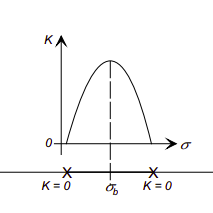
\includegraphics[width=40mm,scale=0.4]{K_graph}$$
    The breakaway points occur at 
    $$\frac{d K}{d \sigma}=-\frac{d}{d K}\left(\frac{D(\sigma)}{N(\sigma)}\right)=0$$
    $$K=\frac{-\left(s^{2}+2 s+5\right)}{6 s}=-\frac{1}{6}\left[s+2+\frac{5}{s}\right]$$
    
\end{frame}
\begin{frame}{Final Result}
    And,
    $$\frac{d k}{d s}=0 \Rightarrow\left[1-\frac{5}{s^{2}}\right]=0$$ 
    Solving for s, we get
    $$s^{2}-5=0 \Rightarrow s=\pm \sqrt{5}$$
    Since, 's' can only be in left half of plane 
    $$\boxed{s=-\sqrt{5}}$$
    $$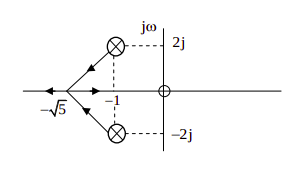
\includegraphics[width=50mm,scale=0.5]{poles_graph}$$
\end{frame}
\begin{frame}{Root Locus Plot}
    $$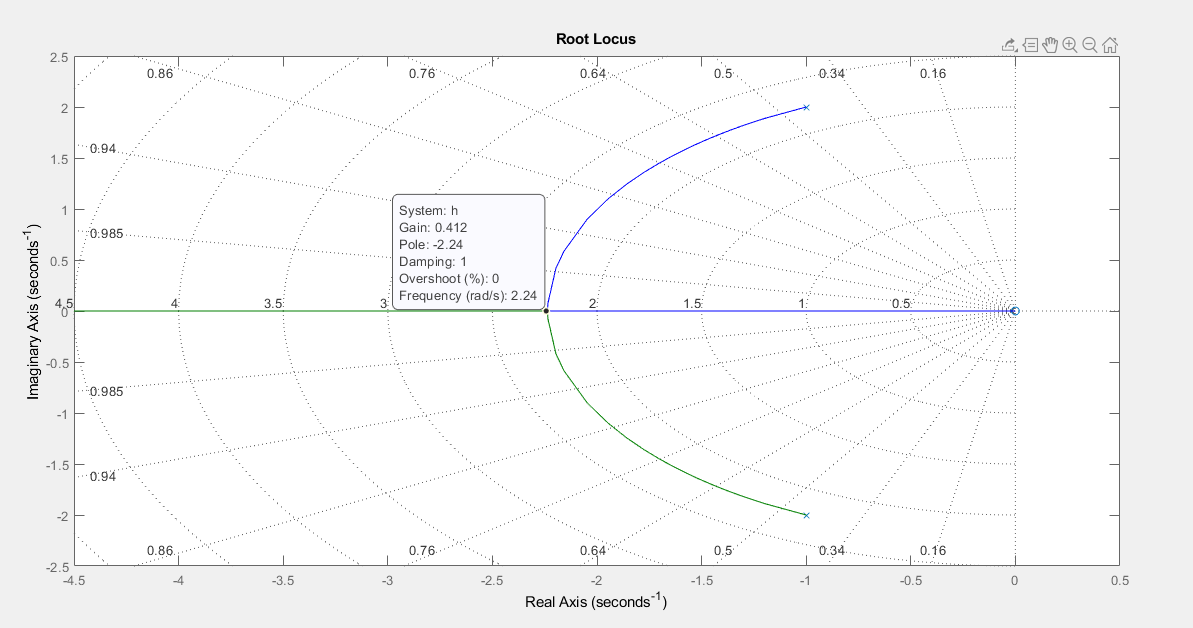
\includegraphics[scale = 0.37]{RL.png}$$
\end{frame}


\end{document}
